%%% LaTeX Template
%%% This template can be used for both articles and reports.
%%%
%%% Copyright: http://www.howtotex.com/
%%% Date: February 2011

%%% Preamble
\documentclass[paper=a4, fontsize=11pt]{scrartcl}	% Article class of KOMA-script with 11pt font and a4 format


\usepackage[italian]{babel}															% English language/hyphenation
\usepackage[protrusion=true,expansion=true]{microtype}				% Better typography
\usepackage{amsmath,amsfonts,amsthm}										% Math packages
\usepackage[pdftex]{graphicx}														% Enable pdflatex
%\usepackage{color,transparent}													% If you use color and/or transparency
\usepackage[hang, small,labelfont=bf,up,textfont=it,up]{caption}	% Custom captions under/above floats
\usepackage{epstopdf}																	% Converts .eps to .pdf
\usepackage{subfig}																		% Subfigures
\usepackage{booktabs}																	% Nicer tables
\usepackage[utf8x]{inputenc} 
\usepackage{listings}
\usepackage{xcolor}
\usepackage[hidelinks]{hyperref}

\lstdefinestyle{sharpc}{language=[Sharp]C, frame=lr, rulecolor=\color{blue!80!black}}

  \usepackage{courier}

%%% Advanced verbatim environment
\usepackage{verbatim}
\usepackage{fancyvrb}
\DefineShortVerb{\|}								% delimiter to display inline verbatim text


%%% Custom sectioning (sectsty package)
\usepackage{sectsty}								% Custom sectioning (see below)
\allsectionsfont{%									% Change font of al section commands
	\usefont{OT1}{bch}{b}{n}%					% bch-b-n: CharterBT-Bold font
%	\hspace{15pt}%									% Uncomment for indentation
	}

\sectionfont{%										% Change font of \section command
	\usefont{OT1}{bch}{b}{n}%					% bch-b-n: CharterBT-Bold font
	\sectionrule{0pt}{0pt}{-5pt}{0.8pt}%	% Horizontal rule below section
	}


%%% Custom headers/footers (fancyhdr package)
\usepackage{fancyhdr}
\pagestyle{fancyplain}
\fancyhead{}														% No page header
\fancyfoot[C]{\thepage}										% Pagenumbering at center of footer
\renewcommand{\headrulewidth}{0pt}				% Remove header underlines
\renewcommand{\footrulewidth}{0pt}				% Remove footer underlines
\setlength{\headheight}{13.6pt}

%%% Equation and float numbering
\numberwithin{equation}{section}															% Equationnumbering: section.eq#
\numberwithin{figure}{section}																% Figurenumbering: section.fig#
\numberwithin{table}{section}																% Tablenumbering: section.tab#


\definecolor{pblue}{rgb}{0.13,0.13,1}
\definecolor{pgreen}{rgb}{0,0.5,0}
\definecolor{pred}{rgb}{0.9,0,0}
\definecolor{pgrey}{rgb}{0.46,0.45,0.48}


\usepackage{color}
\usepackage{xcolor}
\usepackage{listings}

 \lstset{
         basicstyle=\footnotesize\ttfamily, % Standardschrift
         %numbers=left,               % Ort der Zeilennummern
         numberstyle=\tiny,          % Stil der Zeilennummern
         %stepnumber=2,               % Abstand zwischen den Zeilennummern
         numbersep=5pt,              % Abstand der Nummern zum Text
         tabsize=2,                  % Groesse von Tabs
         extendedchars=true,         %
         breaklines=true,            % Zeilen werden Umgebrochen
         keywordstyle=\color{red},
    		frame=b,         
 %        keywordstyle=[1]\textbf,    % Stil der Keywords
 %        keywordstyle=[2]\textbf,    %
 %        keywordstyle=[3]\textbf,    %
 %        keywordstyle=[4]\textbf,   \sqrt{\sqrt{}} %
         stringstyle=\color{white}\ttfamily, % Farbe der String
         showspaces=false,           % Leerzeichen anzeigen ?
         showtabs=false,             % Tabs anzeigen ?
         xleftmargin=17pt,
         framexleftmargin=17pt,
         framexrightmargin=5pt,
         framexbottommargin=4pt,
         %backgroundcolor=\color{lightgray},
         showstringspaces=false      % Leerzeichen in Strings anzeigen ?        
 }

\usepackage{caption}
\DeclareCaptionFont{white}{\color{white}}


%%% Title	
\title{ \vspace{-1in} 	\usefont{OT1}{bch}{b}{n}
		\huge \strut Implementazione di Finding Triangles con Hadoop MapReduce\strut \\
		\Large \bfseries \strut Sistemi di elaborazione di grandi quantità di dati 2016 \strut
}
\author{ 									\usefont{OT1}{bch}{m}{n}
        Nicola Febbrari\\		\usefont{OT1}{bch}{m}{n}
        Università degli Studi di Verona\\	\usefont{OT1}{bch}{m}{n}
        Facoltà di Scienze\\
        \texttt{nicola.febbrari@studenti.univr.it}\\
        \href{https://github.com/nickxbs/LabBigData}{https://github.com/nickxbs/LabBigData}
}
\date{21 giugno 2017}

%%% Begin document
\begin{document}
\maketitle
\section{Introduzione}
Lo scopo del progetto è quello di implementare un algoritmo per calcolare il numero di triangoli presenti in un grafo non diretto, utilizzando le tecniche di MapReduce e il Framework Haddop.


\section{Il problema}
I social network negli ultimi anni hanno avuto una notevole diffusione, l'aumento del numero di utenti che interagiscono con questi sistemi ha avuto come conseguenza un  incremento della quantità di dati che devono essere registrati, gestiti ed ovviamente elaborati.\\
Un social network può essere rappresentato matematicamente da un grafo e una caratteristica molto interessante di questo grafo è il numero di triangoli\footnote{Dati 3 nodi (A,B,C) in un grafo, se un nodo A è collegato con un arco sia con B che con C, nel grafo viene a formarsi un triangolo se esiste anche l'arco che lega B con C.} 
contenuti in esso. Questo numero, rapportato al totale dei triangoli che esisterebbero con una distribuzione casuale e uniforme delle relazioni, può essere un indice di quanto sia social il grafo analizzato.\\
Gli algoritmi sviluppati prendono in considerazioni grafi non diretti.\\
\section{Strumenti e Framework}
\paragraph{Infrastruttura}
Per semplicità e rapidità di configurazione ho deciso di utilizzare Claudera come distribuzione di Hadoop nella sua versione per Docker.
\paragraph{Sviluppo}
Dovendo utilizzare il Framework Hadoop il programma è stato scritto in Java utilizzando le API di Hadoop 2.6 e come IDE di sviluppo ho utilizzato IntelliJ.  

\paragraph{Versioning}
Come sistema di versioning ho utilizzato Git e GitHub come spazio di hosting dei sorgenti.
\footnote{\href{https://github.com/nickxbs/LabBigData}{https://github.com/nickxbs/LabBigData}}


\section{Implementazioni}
\subsection{Algoritmo 2 Jobs}
L'algoritmo a 2 Jobs prevede un prima fase in cui vengono elaborate tutte le relazioni e viene creata in output la combinazione di tutti i possibili triangoli a meno dell'ultimo arco necessario per chiudere il triangolo.\footnote{L'arco mancante è quello fra i 2 nodi maggiori del triangolo dove la relazione d'ordine del nodo è data dall'identificativo del nodo stesso} \\


\begin{figure}[h]
\centering
        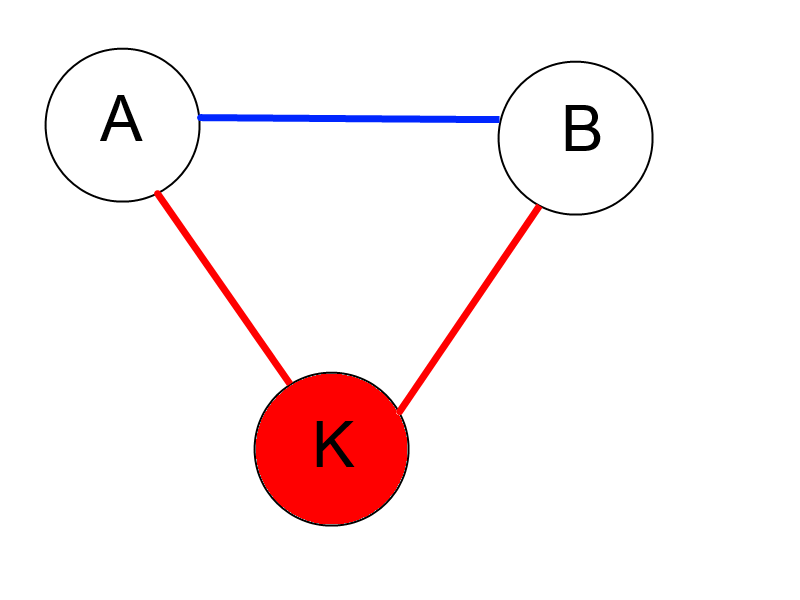
\includegraphics[totalheight=6cm]{Graph1.png}
    \caption{Il Job 1 elabora le relazioni rosse in cui K è il nodo minore del triangolo. Il Job2 cerca la relazione blu A B.}
    \label{fig:verticalcell} 
\end{figure}
\paragraph{Job1 Mapper}
Il grafo da analizzare è rappresentato da un file di testo in cui ogni nodo è identificato da un numero intero e ogni riga rappresenta la relazione fra due nodi.\\
Il Mapper del primo Job carica il grafo e per ogni relazione contenuta in esso emette in output una copia \textit{chiave-valore}, in cui la chiave è il nodo minore e il valore è il nodo maggiore.

\paragraph{Job1 GroupComparator}
Il GroupComparator raggruppa tutte le coppie generate dal Mapper e, per ogni possibile chiave, crea una lista con i valori delle coppie aventi la stessa chiave
\paragraph{Job1 Reducer}

Il Reducer elabora l'input raggruppato dal GroupComparator e, per ogni valore in cui \textit{K} è chiave, costruisce una lista \textit{list} in cui aggiunge tutti i valori prodotti dal Mapper abbinati a \textit{K}.\\
Quando la costruzione di \textit{list} è terminata e tutti i valori abbinati alla chiave \textit{K} sono stati inseriti, esegue il processo di scrittura dell'output delle coppie \textit{chiave-valore} in cui le chiavi sono date dalla combinazione di tutte le possibili coppie di valori presenti in \textit{list}, mentre il valore è il nodo \textit{K}.

\paragraph{Job2 Mapper}
Il Mapper del secondo Job unisce l'output del primo Job al grafo iniziale. Se l'elemento in INPUT A-B è una relazione di quelle presenti nel grafo iniziale, scrive in output un elemento \textit{chiave-valore} con una chiave strutturata (A-B,false) e come valore 0, se invece l'input è una coppia \textit{chiave-valore} (A-B)-V generata dal Job 1, scrive in output un elemento con chiave (A,B,true) e valore V.
\paragraph{Job2 GroupComparator}
Il secondo GroupComparator raggruppa tutti gli elementi generati dal Mapper, mettendo insieme quelli che hanno la stessa prima parte di chiave (A-B), indipendentemente dal valore booleano che viene utilizzato solo per l'ordinamento degli elementi da sottoporre al Reducer.

\paragraph{Job2 Reducer}
Il secondo Reducer, per ogni iterazione, analizza una chiave (A-B) che raggruppa i valori sia di (A-B,false) che di (A-B,true). Se come primo elemento trova un (A-B,false), allora tutti i valori successivi positivi sono nodi che chiudono un triangolo. Se invece il primo nodo analizzato ha chiave (A,B,true) allora l'iterazione del gruppo (A,B) può essere completamente saltata.
\subsection{Algoritmo 5 Jobs}
L'algoritmo a 5 Jobs prevede prima una fase in cui i primi 2 Jobs calcolano il totale dei degli archi e il grado di ogni singolo nodo, queste informazioni poi verranno usate nei successivi 3 Jobs, i quali andranno ad eseguire il calcolo dei triangoli.
\paragraph{Job 1}
Il primo Job è molto semplice e per ogni arco emette un valore 1. Il Reducer conta tutti questi valori, ne fa la somma che poi scrive come output, questo valore rappresenta la quantità di nodi presenti nel grafo.
\paragraph{Job 2}
Il Mapper del secondo Job per ogni relazione A-B emette 2 valori A-1 e B-1.\\
Le funzioni di Grouping e il Partitioner mi garantiscono che tutti i valori di uno stesso nodo vengano accumulati nello stesso Reducer e nello stesso ciclo iterativo. Completato il ciclo scrive in output, per ogni nodo, la somma di tutti i valori emessi dal Mapper, questo valore rappresenta il grado del nodo.
\paragraph{Job 3}
Nella seconda fase viene eseguito l'algoritmo vero e proprio.\\
Obiettivo del Job 3 è di trovare tutti i triangoli che sono composti da nodi \textit{Heavy Hitter}, ovvero con un grado maggiore di $\sqrt{} m$ dove m è il numero degli archi del grafo.\\
Il Mapper, utilizzando il lavoro dei Jobs precedenti, costruisce in memoria un indice di nodi \textit{Heavy Hitter} ed esclude dall' analisi tutti i nodi non nell' indice.\\
Definita una relazione $\prec$ di ordinamento dei nodi in base al grado, si può assumere che ogni triangolo sia formato da 3 nodi (X,Y,Z) i quali sono legati dalle 3 relazioni \textit{tipo A} (X,Y) con X$\prec$Y, \textit{tipo B} (X,Z) con X$\prec$Z e \textit{tipo C} (Y,Z) con Y$\prec$Z.\\
Ogni relazione presente nel grafo può essere una delle 3 che compongono il triangolo, quindi se R=(U,V) una relazione che appartiene ad un triangolo allora sarà di \textit{tipo A} e quindi  il triangolo sarebbe (U,V,?) oppure \textit{tipo B}con (U,?,V) o di \textit{tipo C} con (?,U,V).\\
Il task di Map per sfruttare il parallelismo dei Reducer divide l'input in tante parti quante le possibili combinazioni in cui ogni relazione può essere utilizzata per completare un triangolo.\\
Per implementare questa suddivisione, viene definita una funzione di hash \textit{h} e un parametro \textit{b} che indica quanti sono i possibili valori in output della funzione. In base a questo parametro ogni relazione di input R(X,Y) viene distribuita in 3bk Reducers utilizzando la funzione \textit{H} e seguendo questo schema: (\textit{h}(X),\textit{h}(Y),1$\leq$i$\leq$b) ipotizzando che R sia di \textit{tipo A} , (\textit{h}(X),1$\leq$i$\leq$b,\textit{h}(Y)) se R fosse di \textit{tipo B} e (1$\leq$i$\leq$b,\textit{h}(X),\textit{h}(Y)) se R fosse di \textit{tipo C}. Ogni relazione R viene inclusa in tutti i possibili Reducer in cui potrebbe essere utilizzata per il completamento di un triangolo.\\
Il Reducer, dopo una opportuna ridefinizione delle classi di Gruouping e Ordinamento, scorrere tutti gli elementi in input. L'ordinamento è definito in modo da analizzare, per ogni nodo \textit{K}, prima le possibili relazioni di \textit{tipo A}, per ognuna di esse viene inserito il nodo destinazione \textit{A} in una Lista \textit{listK}. Successivamente vengono analizzate le relazioni di \textit{K} di \textit{tipo B} con \textit{B} come nodo di destinazione, per ognuna di esse viene creata una Map \textit{mapPairK} in cui la chiave è la copia formata da ogni elemento di \textit{listK} e \textit{B} e il valore è il nodo \textit{K}.
L'analisi successiva della relazione di \textit{tipo C} fra \textit{A'} e \textit{B'}, se nella \textit{mapK} esiste una chiave formata dalla coppia  \textit{A',B'} con valore e allora nel grafo esisterà un triangolo \textit{K,A',B'}.
L'ordinamento con cui viene eseguita questa analisi consente di ottimizzare lo spazio di memoria utilizzato e ci garantisce che ogni triangolo venga rilevato solo una volta.
\paragraph{Job 4}
Il Job 4 è molto simile al Job3, l'unica differenza è che in questo caso si vogliono escludere tutti i triangoli di tipo \textit{Heavy Hitter} già calcolati in precedenza.\\
Data una relazione X,Y se X è \textit{Heavy Hitter} X,Y potrebbe appartenere ad un triangolo non \textit{Heavy Hitter} se solo se X,Y è di \textit{tipo C}. Infatti per la relazione di ordinamento $\prec$ definita precedentemente dato il triangolo T(X,Y,?) in cui X,Y è di \textit{tipo A}, qualsiasi ? e Y sarebbero maggiori di X e quindi T sarebbe \textit{Heavy Hitter}, la stessa cosa se X,Y fosse di \textit{tipo B}.\\
Grazie a questa caratteristica il Mapper esclude le relazioni di \textit{tipo A} e \textit{tipo B} in cui \textit{X,Y} ha \textit{X} \textit{Heavy Hitter}.
Il Reducer, a differenza di quello utilizzato in precedenza non usa la Map per salvare i risultati intermedi ma li emette come output insieme a tutte le relazioni \textit{tipo C}.
\paragraph{Job 5}
Completa l'algoritmo controllando se, per ogni elemento calcolato dal Job4, esiste un arco di \textit{tipo C} che chiuderebbe il triangolo.
\section{Sviluppo}
\subsection{Prima iterazione} 
Durante la prima iterazione implementativa ho realizzato l'algoritmo a 2 Job che mi è risultato semplice dal punto di vista implementativo e mi ha aiutato a familiarizzare con il paradigma Map reduce e il framework Hadoop. Purtroppo l'algoritmo dal punto di vista computazionale non si completava nemmeno con grafi anche di medie dimensioni.
\subsection{Seconda iterazione} 
Nella seconda iterazione ho implementato l'algoritmo presente nel libro \textit{Mining of Massive Datasets}.\\
Inizialmente mi sono focalizzato sull'implementazione della suddivisione nei vari Bucket ed in un secondo momento ho completato il lavoro scrivendo l'algoritmo per il calcolo dei triangoli. Purtroppo, nonostante i miglioramenti nella velocità dell'algoritmo, anche questa implementazione aveva dei problemi. Dovendo mantenere Liste e Hashtable in memoria con grafi di grandi dimensioni il processo si interrompeva.
\subsection{Terza iterazione} 
Nella terza iterazione ho analizzato le strutture in memoria più pesanti e ho deciso di introdurre un Job intermedio. Con questa implementazione sono riuscito ad elaborare anche grafi di grandi dimensioni.\\ 
Durante l'analisi di alcuni risultati sul cluster ho riscontrato un bug molto evidente. Il bug era causato dalle dimensioni del file contenente il grado dei nodi, questo per grafi molto grandi veniva suddiviso su più Mapper e quindi in alcuni casi risultava parziale.
\subsection{Conclusione} 
Nell'ultima iterazione ho corretto il bug introducendo delle DistributedCache che mi consentivano di vincolare il caricamento dell'intero file dei gradi dei nodi su ogni singolo Mapper. Inoltre ho aggiunto delle classi di Helper per agevolarmi nel testing e nel debugging dei singoli Job.
\section{Risultati}
\subsection{Social circles: Facebook\protect\footnote{http://snap.stanford.edu/data/egonets-Facebook.html}} 
\protect\begin{table}[]
	\centering
	\caption{Facebook}
	\label{my-label}
	\begin{tabular}{ll}
		Nodi		 & 4039 \\
		Archi		 & 88234 \\
		Triangoli	& 1612010 \\
	\end{tabular}
\end{table}
Riferimenti:\\	
\href{http://hadoop-compute0.di.univr.it:50030/jobdetails.jsp?jobid=job_201603141010_12286}{Job1}\\
\href{http://hadoop-compute0.di.univr.it:50030/jobdetails.jsp?jobid=job_201603141010_12287}{Job2}\\
\href{http://hadoop-compute0.di.univr.it:50030/jobdetails.jsp?jobid=job_201603141010_12288}{Job3}\\
\href{http://hadoop-compute0.di.univr.it:50030/jobdetails.jsp?jobid=job_201603141010_12289}{Job4}\\
\href{http://hadoop-compute0.di.univr.it:50030/jobdetails.jsp?jobid=job_201603141010_12290}{Job5}\\

\subsection{Amazon product co-purchasing network and ground-truth communities\protect\footnote{http://snap.stanford.edu/data/com-Amazon.html}} 
\protect\begin{table}[]
	\centering
	\caption{Amazon}
	\label{my-label}
	\begin{tabular}{ll}
		Nodi		 & 334863 \\
		Archi		 & 925872 \\
		Triangoli	& 667129 \\
	\end{tabular}
\end{table}
Riferimenti:\\	
\href{http://hadoop-compute0.di.univr.it:50030/jobdetails.jsp?jobid=job_201603141010_12271}{Job1}\\
\href{http://hadoop-compute0.di.univr.it:50030/jobdetails.jsp?jobid=job_201603141010_12272}{Job2}\\
\href{http://hadoop-compute0.di.univr.it:50030/jobdetails.jsp?jobid=job_201603141010_12273}{Job3}\\
\href{http://hadoop-compute0.di.univr.it:50030/jobdetails.jsp?jobid=job_201603141010_12274}{Job4}\\
\href{http://hadoop-compute0.di.univr.it:50030/jobdetails.jsp?jobid=job_201603141010_12275}{Job5}\\

\subsection{Youtube social network\protect\footnote{http://snap.stanford.edu/data/com-Youtube.html}} 

\begin{table}[]
	\centering
	\caption{Youtube}
	\label{my-label}
	\begin{tabular}{ll}
		Nodi		 & 1134890\\
		Archi		 & 2987624 \\
		Triangoli	& 3056386 \\
	\end{tabular}
\end{table}
Riferimenti:\\	
\href{http://hadoop-compute0.di.univr.it:50030/jobdetails.jsp?jobid=job_201603141010_12281}{Job1}\\
\href{http://hadoop-compute0.di.univr.it:50030/jobdetails.jsp?jobid=job_201603141010_12282}{Job2}\\
\href{http://hadoop-compute0.di.univr.it:50030/jobdetails.jsp?jobid=job_201603141010_12283}{Job3}\\
\href{http://hadoop-compute0.di.univr.it:50030/jobdetails.jsp?jobid=job_201603141010_12284}{Job4}\\
\href{http://hadoop-compute0.di.univr.it:50030/jobdetails.jsp?jobid=job_201603141010_12285}{Job5}\\

\section{Sviluppi futuri}
Mi sarebbe piaciuto completare il progetto generando come artefatto del processo un immagine Docker pronta all'uso \protect\footnote{Una prima versione è disponibile su https://hub.docker.com/r/nickxbs/labbigdata }. Sarebbe interessante provare a fare un deploy per testare questo container in un ambiente cloud che supporta Docker.\\
Un secondo aspetto che mi sarebbe piaciuto approfondire è l'uso di un framework di Unit testing per Hadoop. L'unico che ho provato velocemente è Mrunit, tuttavia il progetto sembra non essere più mantenuto.
\end{document}